\chapter{Experiments}
\label{ch:experiments}
At first we provide a brief intro about our setup, including the used software, preprocessing, \gls{dl} models, and applied parameters. Secondly we cover the experiments, which are divided into two parts:
\begin{itemize}
    \item \textbf{Test experiments}: We try to understand how in general the \gls{dl} models could classify only the syllables, without additional background samples.
    \item \textbf{Seq experiments}: We investigate the \gls{dl} models' performance on detecting syllables by providing the whole audio as slices in a moving window manner.
\end{itemize}

\section{Main setup}
This chapter contains the general experiment set-up. Specialisations are described in the additional subchapters in the individual experiment chapters if required.

\subsection{Software}
We adapted a piece of software created with the bachelor thesis "Bird Voice Deep Learning" \cite{Waeber2019BirdLearning} kindly provided by Gilles Waeber.
Apart from needing a similar pipeline and \gls{dl} models to conduct our experiments, it provides some interesting features like interruption awareness and extended logging of the results in an accessible manner.

\subsubsection{Changes}
We removed the birdvoice\_server section of the code and everything else needed to run the web application.
The Docker files we kept back, but they would first have to be adapted to the new folder structure.
Since UBELIX, the HPC cluster at the University of Bern, does not directly support docker, we did not further invest in it.
Moreover, due to the possibility of installing our custom software on UBELIX, we no longer needed this or similar options.

Then we updated to TensorFlow 2.3, as with this version we could use the Ragged Tensors for variable length input data.
This allowed us to train the \gls{lstm} model through the convenient training method from Keras-Model including batch and \gls{gpu} support. Therefore, we could ignore all the specialized parts of the software written for training the \gls{rnn} models with variable length input.

For portability reasons, all file paths are made relative to the data path and converted to slash delimited paths which are written to reports or similar reused data files.

We used the jupyter notebook library for generating reports about the experiment testing results. The reports are generated by a template which can be customized as needed.

\subsubsection{Dependencies}
Over time and with the advent of new products or simply through convenience, the dependencies have changed a little.
The changes are presented below:
\begin{itemize}
    \item Python 3.8, although unfortunately we do not make direct use of new features such as the walrus operator.
    \item TensorFlow, this version enables faster \gls{lstm} training, as it fully supports the concept of Ragged Tensor.
    \item innvestigate\@updates\_towards\_tf2.0, with some additional modifications, we could use the "innvestigate" library in conjunction with TensorFlow 2.3 for generating the \gls{lrp} headmaps by the deeptalyor algo.
    \item Wavinfo 1.6.2, is used for extracting the label information produced by the avisoft software.
\end{itemize}

\noindent
Below are the relevant python libraries:
\begin{itemize}
\pyLib{TensorFlow GPU 2.3.1}{https://www.tensorflow.org/}{machine learning backend}{Apache 2.0}{https://github.com/tensorflow/tensorflow/blob/master/LICENSE}
\pyLib{Numpy 1.19.1}{https://numpy.org/}{fast numeric computation}{BSD-3-Clause}{https://github.com/numpy/numpy/blob/master/LICENSE.txt}
\pyLib{TQDM 4.50.2}{https://github.com/tqdm/tqdm}{progress bars}{MPL 2.0}{https://github.com/tqdm/tqdm/blob/master/LICENCE}
\pyLib{SciPy 1.5.3}{https://scipy.org/}{linear algebra}{BSD-3-Clause}{https://github.com/scipy/scipy/blob/master/LICENSE.txt}
\pyLib{Matplotlib 3.3.1}{https://matplotlib.org/}{2D plotting}{PSF}{https://matplotlib.org/users/license.html}
\pyLib{FileLock 3.0.12}{https://github.com/benediktschmitt/py-filelock}{file locking}{Unlicense}{https://github.com/benediktschmitt/py-filelock/blob/master/LICENSE}
\pyLib{Jupyter Notebook 4.6.3}{https://jupyter-notebook.readthedocs.io/}{interactive notebooks}{BSD-3-Clause}{https://github.com/jupyter/notebook/blob/master/LICENSE}
\pyLib{Librosa 0.8.0}{https://librosa.org/doc}{manipulate audio}{ISC License}{https://github.com/librosa/librosa/blob/main/LICENSE.md}
\pyLib{Wavinfo 1.6.2}{https://wavinfo.readthedocs.io}{read wav labels}{MIT License}{https://github.com/iluvcapra/wavinfo/blob/master/LICENSE}
\end{itemize}

\subsection{Spectrogram}
\begin{itemize}
\item The spectrograms have been created with SoX using the audio recordings.
\item Sampling rate is set to \SI{500}{\kHz}.
\item Height is variable, no band-pass filtering (0-\SI{250}{\kHz}).
\item All other parameters vary per experiments.
\end{itemize}

\subsection{Samples}
\begin{itemize}
\item The models were trained by k-fold cross-validation with k = 8, validation bins 1 and testing bins 2.
\item The samples are distributed among the bins so that each bin contains the same number of samples for each class. The remaining samples are always used for training and therefore do not change between runs.
\end{itemize}

\subsection{Features}
\begin{itemize}
% normalizing is more mean 0 and sd +-1 or putting different variables on a common scale.
% -> scaling fits here more
\item Raw stands for pixel features from the spectrogram scaled between 0 and 1. % the scale is because of the matplotlib
\item For \gls{hog} features, the descriptors are extracted by HWRecog (without preprocessing) using the Slit-Style \gls{hog} variant.
\item The \gls{hog} variant suffixed with 3D, the 12 bins of the HOG-descriptor are populated to 12 channels/layers of the image.
\item The values are normalized for each sample between -1 and 1.
\end{itemize}

\subsection{LSTM Model}
\begin{figure}[ht!]
\centering
  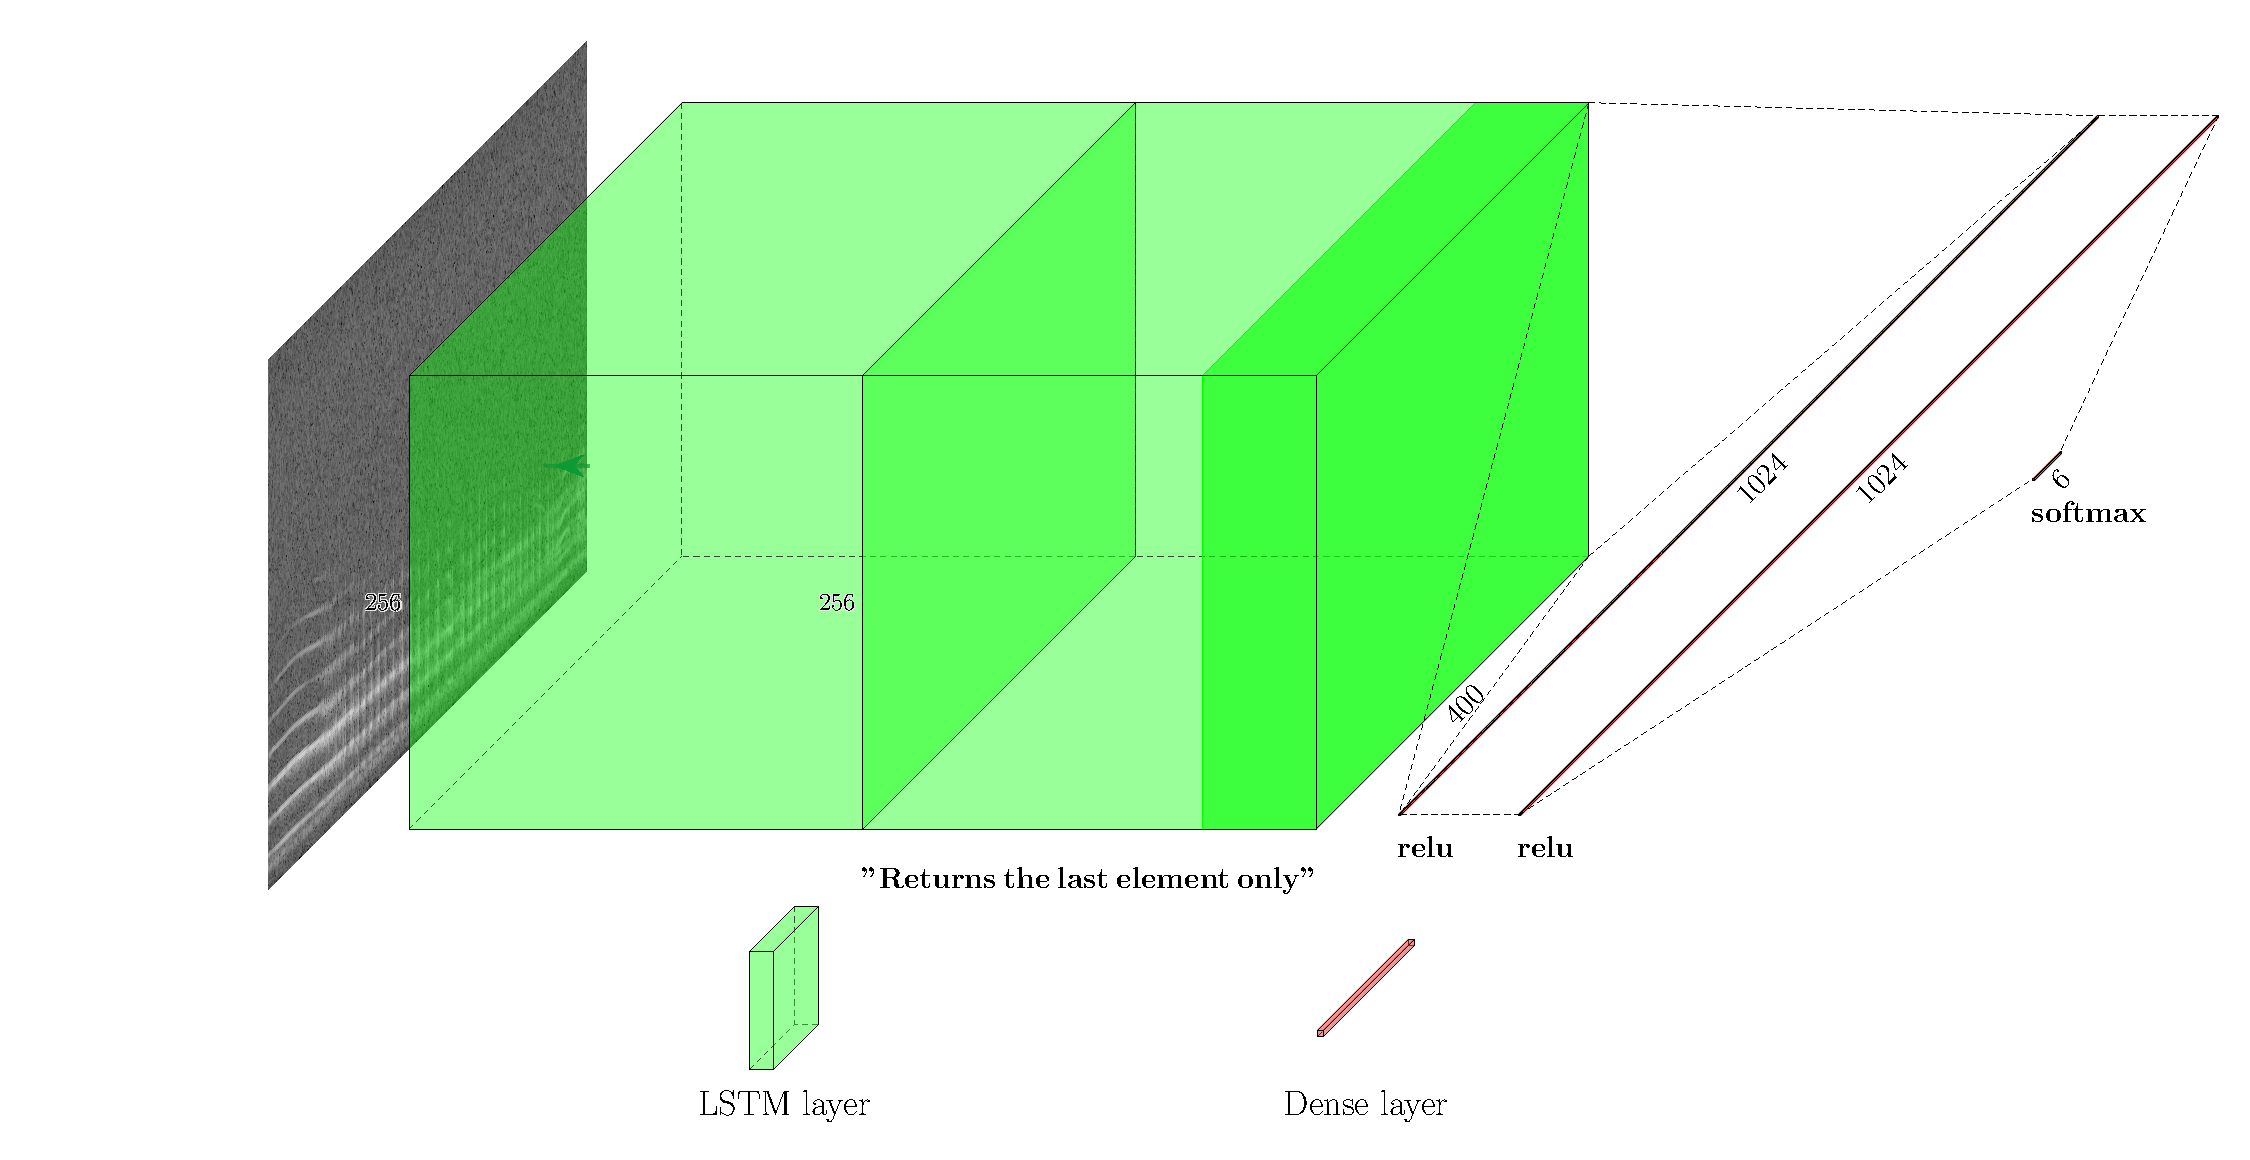
\includegraphics[width=0.9\textwidth]{image/model/ml_model_lstm.pdf}\hfill
  \caption{Visualisation of the \gls{lstm} architecture. The size of the elements does not correspond exactly to their real dimension numbers.}
  \label{fig:ml_model_lstm}
\end{figure}

The \figref{ml_model_lstm} represents the \gls{lstm} architecture used for the experiments. Form left to right:
\begin{itemize}
\item Input layer, it provides raw or \gls{hog} features in various sizes.
\item First \gls{lstm} layer with 265 neurons, it transmits the whole output sequence to the next layer.
\item Second \gls{lstm} layer with 265 neurons. Only the output of the last element is transmitted.
\item Two fully connected layers with 1024 neurons and a dropout rate of 50\%. Both use the ReLU activation function.
\item The final classification layer is a fully connected layer with softmax activation.
\end{itemize}

\subsection{CNN Model}
\begin{figure}[ht!]
\centering
  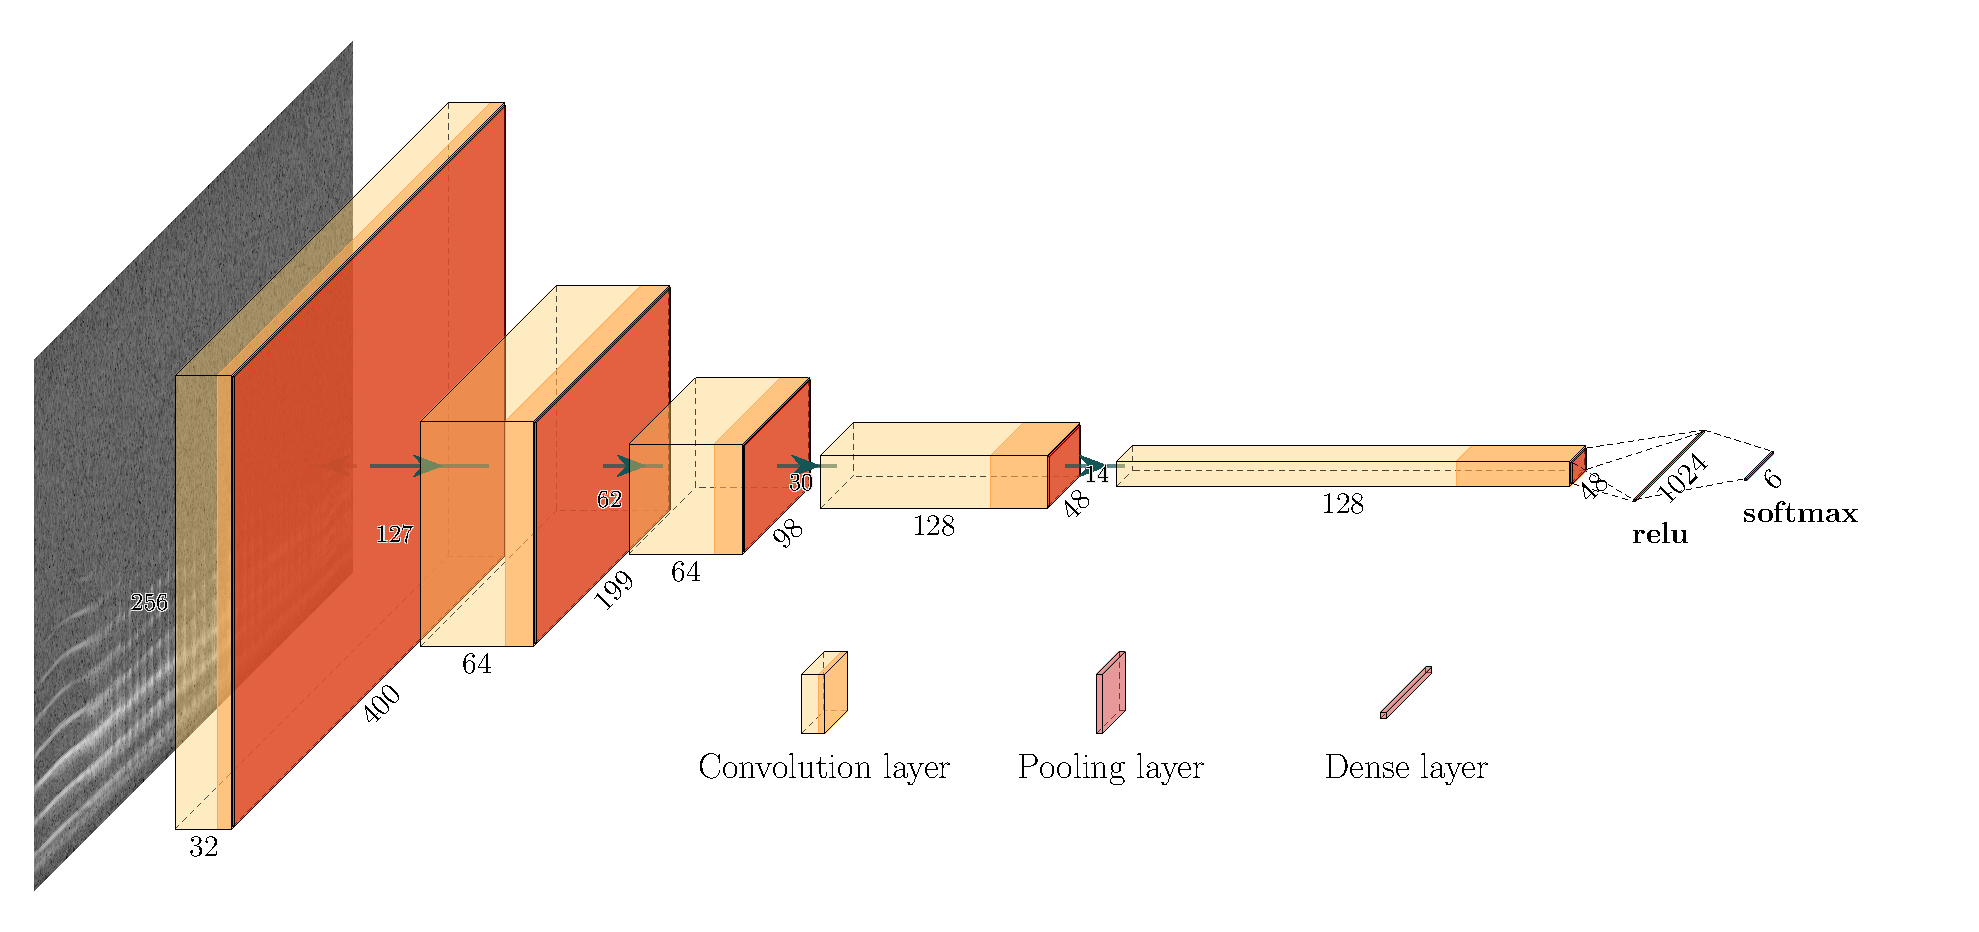
\includegraphics[width=0.9\textwidth]{image/model/ml_model_cnn.pdf}\hfill
  \caption{Visualisation of the CNN architecture. The size of the elements do not correspond exactly to their real dimension numbers.}
  \label{fig:ml_model_cnn}
\end{figure}

The \figref{ml_model_cnn} represents the CNN architecture used for the experiments. Where the CNN 1D model uses 1 dimensional convolution layers. From left to right:
\begin{itemize}
\item Input layer, it provides raw or \gls{hog} features in various sizes. % dimensions or sizes???
\item The next five blocks consist of a convolution layer followed by a max pooling layer with ReLU activation function.
The size and stride of the pooling layer are $2\times2$, resulting in dividing the size of the volume and the number of feature maps in half.
From the second block onwards the next block is only created if the output shape of the previous block is big enough.
The filter configurations of the convolution layer in the blocks are as follows:
    \begin{enumerate}
    \item $32\times3\times3$
    \item $64\times3\times3$
    \item $64\times3\times3$
    \item $128\times3\times3$
    \item $256\times3\times3$
    \end{enumerate}
\item The output of the previous max pooling layer is flattened (sample dimension reduced to one) and transmitted to a fully connected layer with 1024 neurons, a dropout rate of 50\% and a ReLU activation function.
\item The final layer, also called the classification layer, is a fully connected layer with the same number of neurons as classes. The classification layer uses the softmax activation function.
\end{itemize}

\subsection{DenseNet Model}
We use the DenseNet-121 architecture as described here \cite{Huang2017a} followed by a a fully connected layer with 1024 neurons, a dropout rate of 50\% and a ReLU activation function. The final classification layer uses the softmax activation function.

\section{Test experiments}
The general aim of these experiments is to understand how the models performs on different preprocessed syllable samples. Therefore, we only altered the preprocessing hyperparameters for the different tests.
However, one should be aware that the gls{dl} models are automatically adjusted to the size of the input data, which leads to a change in the number of parameters of a gls{dl} model.
Whenever possible, we tested the resulting features on all \gls{dl} models.

\subsection{Specialized setup}
For all test experiments, the source of the data remained the same.
Unfortunately, constraint by the spectrogram resolution and feature type applied, we had to exclude some syllable types in some experiments.

\subsubsection{Cutting the syllables}
The syllable parts are extracted from the audio source based on their start and end times, the SOX software was used for this.

\subsubsection{Silent profile and noise reduction}
We generated one silent file per audio file group, from this we created the noise profile and applied it to the extracted syllable audio file with the effect controlled by the sensitivity parameter called \gls{nrs}.
How we defined the silent parts of an audio source is described in \secref{silent_detection}. % muss es "audio source" sein oder reicht audio?

For the manual labelling, the original audio recording was cut into smaller pieces, whereby sub strings from the file name were changed or extended.
We tried to reverse this process as it was sometimes difficult to extract background noise from the edited audio files at all.
The audio file group is defined by a pattern in the file name of the audio files. The extracted pattern is used as the key for grouping the audio files and generating the silent audio file name.

\subsection{Compressed}
% ======= specs ==========
% ----- syllable duration
% min 22.19
% max 200.4
% 200.4/22.19=9,031095088
% -----
The goal for this experiment was to evaluate how well the \gls{dl} models could learn to classify the syllables when they are compressed with respect to the time axes. Additionally, this should give us a sort of baseline of what we should achieve in future optimized runs.
\subsubsection{Setup}
The raw and \gls{hog} features were prepared as follows:
\begin{itemize}
%    \item because it is not simply possible with sox to extract spectrogram images lower than 100 samples (pixel in width) we had to exclude all samples which were smaller than \SI{22}{\milli\second}
    \item Because the version of sox has a minimum fixed width length of 100 pixel, we had to filter out the syllables that were shorter than \SI{22}{\milli\second}.
    This value is \SI{2}{\milli\second} more than should theoretically be possible with sox, since sox has a maximum resolution of 5000 pixels per second, which would allow a minimum length of \SI{20}{\milli\second}.
    However, with samples below \SI{22}{\milli\second}, sox sometimes fails to create the spectrograms in the correct size after noise reduction is applied.
    \item Additionally after filtering the dataset in length, we kept all syllable types with a minimum sample count of 50 samples.
    This resulted in a smaller dataset, where the ratio between the shortest and the longest syllable sample is around 1 : 9.
    \item The syllables were extracted.
    \item A noise reduction filter with sensitivity of 6\%, 12\% and 21\% or no noise reduction was applied to the extracted syllables.
    \item Finally, the samples were converted into \num{100 x 256} spectrogram images.
    Compared to the shortest syllable sample, the resulting compression ratio for the largest sample with a duration of \SI{200.4}{\milli\second} is about 1 : 9. The resulting visible change can be seen in the \figref{compressed_spectorgram_b2}.
\end{itemize}

\begin{table}[ht!]
\centering
\begin{tabular}{l
S[table-format=3.2]@{\,\( \pm \)\,}
S[table-format=2.2, table-number-alignment = left]
S[table-format=3.2]
S[table-format=3.2]
S[table-format=3.2]
S[table-format=3]
}
\toprule
syllable type &  \multicolumn{2}{l}{mean/\si{\milli\second}} & {median/\si{\milli\second}} &   {min/\si{\milli\second}} &    {max/\si{\milli\second}} & count \\
\midrule
           B4 & 43.56 & 14.05 &  39.57 & 23.54 &  73.19 &    82 \\
          UPS & 45.45 & 11.13 &  44.07 & 23.04 &  85.59 &   461 \\
           B3 & 54.67 & 17.76 &  53.53 & 26.19 & 120.70 &   124 \\
           B2 & 62.26 & 31.28 &  54.50 & 22.19 & 200.40 &   288 \\
\bottomrule
\end{tabular}

\caption{Descriptive statistic of the syllables used in the compressed experiment.}
\label{tab:syllable_duration_stats_compressed}
\end{table}

\begin{figure}[ht!]
\centering
  \begin{tikzpicture}
  \node (compressed)  {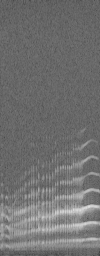
\includegraphics[scale=0.333]{image/generated/compressed_spectorgram_b2_compressed.png}};
  \node[below=of compressed, yshift=32] {\footnotesize 100};
  \node[left=of compressed, node distance=0cm, rotate=90, anchor=center,yshift=-25] {\footnotesize 256};
  \node[below=of compressed, yshift=10] (base)  {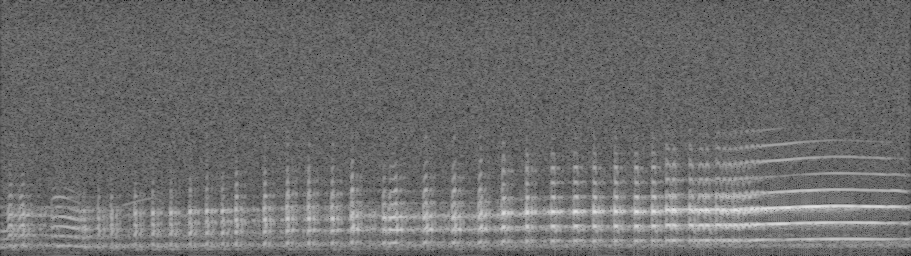
\includegraphics[scale=0.333]{image/generated/compressed_spectorgram_b2.png}};
  \node[below=of base, node distance=0cm, yshift=32] {\footnotesize 911};
  \node[left=of base, node distance=0cm, rotate=90, anchor=center,yshift=-25] {\footnotesize 256};
  \end{tikzpicture}
  \caption{Visualisation of a compression ratio of 1:9 on the basis of the longest syllable sample.}
  \label{fig:compressed_spectorgram_b2}
\end{figure}

As shown in the \figref{dataset_sct_compressed}, the bins contain 10 samples because the smallest set of syllables had only 82 samples. For the syllable type with the most samples, only around 17.35\% of the samples are rotated in the k-fold process. The samples for the bins are taken from the beginning of the data set.

\begin{figure}[ht!]
\centering
  \includesvg[inkscapelatex=false, width=0.7\textwidth]{image/generated/dataset_sct_compressed.svg}\hfill
  \caption{The distribution of the samples used for the compressed test experiment. For all syllables we used 10 samples for validation and 20 for testing. The dataset is not balanced with a ratio of about 1 : 8 in the number of training samples between the least and most represented syllable.}
  \label{fig:dataset_sct_compressed}
\end{figure}

\subsubsection{Results}
\begin{table}[h!]
\centering
\begin{tabular}{l
S[table-format=2.1]@{\,\( \pm \)\,}
S[table-format=1.1, table-number-alignment = left]
S[table-format=2.2]@{\,\( \pm \)\,}
S[table-format=1.2]
S[table-format=2.1]@{\,\( \pm \)\,}
S[table-format=1.1, table-number-alignment = left]
S[table-format=2.2]@{\,\( \pm \)\,}
S[table-format=1.2]
}
\toprule
                                                                                Model & \multicolumn{4}{l}{Validate} & \multicolumn{4}{l}{Test} \\
                                                                                      & \multicolumn{2}{l}{Accuracy (\si{\percent})} & \multicolumn{2}{l}{Loss} & \multicolumn{2}{l}{Accuracy (\si{\percent})} & \multicolumn{2}{l}{Loss} \\

\midrule
            \cite{nn_densNet_sct_compressed_nrs0_raw_100} DenseNet, \gls{nrs}: 0, raw &                     93.4 & 4.2 &     1.23 & 0.75 &                     87.5 &  2.8 &     0.65 & 0.29 \\
               \cite{nn_cnn_2d_sct_compressed_nrs0_raw_100} CNN 2D, \gls{nrs}: 0, raw &                     92.2 & 5.1 &     0.97 & 0.60 &                     87.0 &  4.4 &     0.43 & 0.18 \\
             \cite{nn_cnn_2d_sct_compressed_nrs12_raw_100} CNN 2D, \gls{nrs}: 12, raw &                     91.6 & 5.2 &     0.80 & 0.42 &                     85.6 &  6.0 &     0.41 & 0.14 \\
               \cite{nn_cnn_2d_sct_compressed_nrs6_raw_100} CNN 2D, \gls{nrs}: 6, raw &                     91.2 & 5.5 &     0.87 & 0.43 &                     84.5 &  5.5 &     0.38 & 0.14 \\
          \cite{nn_densNet_sct_compressed_nrs12_raw_100} DenseNet, \gls{nrs}: 12, raw &                     90.9 & 5.2 &     1.51 & 1.26 &                     84.4 &  6.5 &     0.72 & 0.42 \\
             \cite{nn_cnn_2d_sct_compressed_nrs24_raw_100} CNN 2D, \gls{nrs}: 24, raw &                     90.6 & 8.0 &     0.82 & 0.53 &                     84.1 &  5.7 &     0.46 & 0.20 \\
          \cite{nn_densNet_sct_compressed_nrs24_raw_100} DenseNet, \gls{nrs}: 24, raw &                     90.6 & 5.0 &     1.13 & 0.57 &                     83.0 &  4.5 &     0.71 & 0.30 \\
               \cite{nn_cnn_1d_sct_compressed_nrs0_raw_100} CNN 1D, \gls{nrs}: 0, raw &                     90.6 & 4.4 &     1.02 & 0.36 &                     82.7 &  4.7 &     0.49 & 0.08 \\
            \cite{nn_densNet_sct_compressed_nrs6_raw_100} DenseNet, \gls{nrs}: 6, raw &                     91.9 & 5.5 &     1.00 & 0.54 &                     81.2 &  5.6 &     0.66 & 0.31 \\
             \cite{nn_cnn_1d_sct_compressed_nrs24_raw_100} CNN 1D, \gls{nrs}: 24, raw &                     87.5 & 5.7 &     1.18 & 0.57 &                     81.2 &  6.1 &     0.63 & 0.27 \\
               \cite{nn_cnn_1d_sct_compressed_nrs6_raw_100} CNN 1D, \gls{nrs}: 6, raw &                     87.5 & 4.0 &     1.25 & 0.48 &                     79.2 &  2.7 &     0.61 & 0.11 \\
         \cite{nn_cnn_2d_sct_compressed_nrs0_hog_100} CNN 2D, \gls{nrs}: 0, \gls{hog} &                     86.6 & 5.5 &     1.30 & 1.03 &                     79.2 &  4.6 &     0.56 & 0.14 \\
             \cite{nn_cnn_1d_sct_compressed_nrs12_raw_100} CNN 1D, \gls{nrs}: 12, raw &                     86.2 & 5.2 &     1.45 & 0.62 &                     78.4 &  4.3 &     0.68 & 0.15 \\
   \cite{nn_cnn_2d_sct_compressed_nrs0_hog_100_3d} CNN 2D, \gls{nrs}: 0, \gls{hog} 3D &                     83.8 & 3.3 &     1.08 & 0.22 &                     77.7 &  3.7 &     0.54 & 0.05 \\
         \cite{nn_cnn_1d_sct_compressed_nrs0_hog_100} CNN 1D, \gls{nrs}: 0, \gls{hog} &                     85.6 & 3.5 &     1.08 & 0.27 &                     76.9 &  5.1 &     0.57 & 0.06 \\
             \cite{nn_lstm_sct_compressed_nrs0_hog_100} LSTM, \gls{nrs}: 0, \gls{hog} &                     89.7 & 4.9 &     1.24 & 0.39 &                     76.2 &  2.6 &     0.82 & 0.34 \\
      \cite{nn_densNet_sct_compressed_nrs0_hog_100} DenseNet, \gls{nrs}: 0, \gls{hog} &                     87.8 & 2.5 &     1.69 & 1.11 &                     75.8 &  4.4 &     1.20 & 0.21 \\
             \cite{nn_lstm_sct_compressed_nrs6_hog_100} LSTM, \gls{nrs}: 6, \gls{hog} &                     84.1 & 7.3 &     1.78 & 1.10 &                     75.5 &  4.9 &     0.84 & 0.23 \\
         \cite{nn_cnn_2d_sct_compressed_nrs6_hog_100} CNN 2D, \gls{nrs}: 6, \gls{hog} &                     82.8 & 2.1 &     1.61 & 0.98 &                     75.3 &  6.0 &     0.81 & 0.30 \\
           \cite{nn_lstm_sct_compressed_nrs12_hog_100} LSTM, \gls{nrs}: 12, \gls{hog} &                     85.3 & 5.7 &     1.61 & 1.17 &                     73.3 &  6.0 &     0.94 & 0.37 \\
       \cite{nn_cnn_2d_sct_compressed_nrs24_hog_100} CNN 2D, \gls{nrs}: 24, \gls{hog} &                     80.9 & 6.1 &     1.50 & 0.65 &                     73.3 &  9.7 &     0.76 & 0.22 \\
      \cite{nn_densNet_sct_compressed_nrs6_hog_100} DenseNet, \gls{nrs}: 6, \gls{hog} &                     83.1 & 4.2 &     3.12 & 2.26 &                     72.8 &  6.2 &     1.63 & 0.62 \\
       \cite{nn_cnn_2d_sct_compressed_nrs12_hog_100} CNN 2D, \gls{nrs}: 12, \gls{hog} &                     82.5 & 4.0 &     1.22 & 0.42 &                     72.3 &  8.0 &     0.75 & 0.18 \\
       \cite{nn_cnn_1d_sct_compressed_nrs12_hog_100} CNN 1D, \gls{nrs}: 12, \gls{hog} &                     78.4 & 6.5 &     1.52 & 0.58 &                     72.2 &  9.8 &     0.76 & 0.24 \\
 \cite{nn_cnn_2d_sct_compressed_nrs12_hog_100_3d} CNN 2D, \gls{nrs}: 12, \gls{hog} 3D &                     80.6 & 5.8 &     1.30 & 0.46 &                     72.0 &  6.9 &     0.71 & 0.16 \\
         \cite{nn_cnn_1d_sct_compressed_nrs6_hog_100} CNN 1D, \gls{nrs}: 6, \gls{hog} &                     79.7 & 8.3 &     1.40 & 0.55 &                     71.9 &  7.1 &     0.77 & 0.17 \\
                 \cite{nn_lstm_sct_compressed_nrs12_raw_100} LSTM, \gls{nrs}: 12, raw &                     79.1 & 5.5 &     3.84 & 2.41 &                     71.9 &  7.2 &     1.40 & 0.55 \\
           \cite{nn_lstm_sct_compressed_nrs24_hog_100} LSTM, \gls{nrs}: 24, \gls{hog} &                     82.8 & 6.7 &     1.87 & 1.25 &                     71.7 &  8.2 &     0.98 & 0.27 \\
    \cite{nn_densNet_sct_compressed_nrs12_hog_100} DenseNet, \gls{nrs}: 12, \gls{hog} &                     83.1 & 5.1 &     3.62 & 1.49 &                     71.4 &  4.5 &     1.90 & 0.38 \\
   \cite{nn_cnn_2d_sct_compressed_nrs6_hog_100_3d} CNN 2D, \gls{nrs}: 6, \gls{hog} 3D &                     79.7 & 4.9 &     1.57 & 0.48 &                     71.1 &  6.9 &     0.74 & 0.18 \\
                 \cite{nn_lstm_sct_compressed_nrs24_raw_100} LSTM, \gls{nrs}: 24, raw &                     79.1 & 6.4 &     2.76 & 1.09 &                     70.6 &  5.6 &     1.22 & 0.41 \\
    \cite{nn_densNet_sct_compressed_nrs24_hog_100} DenseNet, \gls{nrs}: 24, \gls{hog} &                     77.2 & 6.3 &     3.83 & 1.77 &                     68.9 &  4.9 &     1.77 & 0.28 \\
                   \cite{nn_lstm_sct_compressed_nrs6_raw_100} LSTM, \gls{nrs}: 6, raw &                     76.6 & 5.2 &     3.43 & 1.81 &                     68.4 &  6.9 &     1.26 & 0.63 \\
 \cite{nn_cnn_2d_sct_compressed_nrs24_hog_100_3d} CNN 2D, \gls{nrs}: 24, \gls{hog} 3D &                     78.1 & 6.4 &     1.53 & 0.49 &                     68.0 & 10.2 &     0.79 & 0.22 \\
       \cite{nn_cnn_1d_sct_compressed_nrs24_hog_100} CNN 1D, \gls{nrs}: 24, \gls{hog} &                     78.1 & 6.6 &     1.43 & 0.51 &                     68.0 &  8.8 &     0.89 & 0.24 \\
                   \cite{nn_lstm_sct_compressed_nrs0_raw_100} LSTM, \gls{nrs}: 0, raw &                     77.2 & 4.5 &     2.72 & 1.27 &                     67.7 &  2.3 &     1.23 & 0.52 \\
\bottomrule
\end{tabular}

\caption{Results of the compressed images experiment, sorted by test accuracy.}
\label{tab:result_overview_sct_compressed}
\end{table}
According to the \tabref{result_overview_sct_compressed}, the DenseNet and the \gls{cnn} 2D models perform similar, however the first has a slightly better test accuracy.
Interesting is, that the \gls{cnn} models overcome the visual distortion through the noise reduction and achieve almost similar test accuracy than without.
The \gls{lstm} model becomes even better on the highest \gls{nrs} value when applied to raw features.
However, it should be taken into account that the \gls{lstm} model performs much better on the \gls{hog} features.
And therefore the result about the higher accuracy at high \gls{nrs} in raw values is not further relevant for our goal.

Overall, the \figref{model_distribution_sct_compressed} shows that the \gls{cnn} models perform better than the \gls{lstm} model in terms of raw features. The opposite is true for the \gls{hog} features, but the accuracy is generally lower there. The effect of noise reduction is opposite for the CNN models and the \gls{lstm} model at the raw features. However, the \gls{lstm} model with \gls{hog} features behaves similar to the CNN model with raw features in respect to noise reduction.

\begin{figure}[ht!]
\centering
  \includesvg[inkscapelatex=false, width=0.9\textwidth]{image/generated/train_val_densNet_sct_compressed_nrs0_raw_100.svg}\hfill
  \caption{Training progression for DenseNet model \cite{nn_densNet_sct_compressed_nrs0_raw_100} on raw features.}
  \label{fig:train_val_densNet_sct_compressed_nrs0_raw_100}
\end{figure}

\begin{figure}[ht!]
\centering
  \includesvg[inkscapelatex=false, width=0.9\textwidth]{image/generated/train_val_cnn_2d_sct_compressed_nrs0_raw_100.svg}\hfill
  \caption{Training progression for CNN 2D model \cite{nn_cnn_2d_sct_compressed_nrs0_raw_100} on raw features.}
  \label{fig:train_val_cnn_2d_sct_compressed_nrs0_raw_100}
\end{figure}

Gazing at the learning curves in \figref{train_val_densNet_sct_compressed_nrs0_raw_100} and \figref{train_val_cnn_2d_sct_compressed_nrs0_raw_100}, the best models show an acceptable learning curve with little to no overfitting.
However it can be seen that the \gls{dl} models have difficulty in learning patterns and selecting features that accurately describe the samples in all datasets and tend to overfit. This is revealed by the rather large difference between validation and test accuracy in the result \tabref{result_overview_sct_compressed}.
With the exception of the 2 best models, all others tend to overfit to a greater extent.
This is exemplified in the \figref{train_val_lstm_sct_compressed_nrs0_hog_100}, where the validation loss curve shows a vague U shape and the cap between validation and test accuracy grows until the end.

Even though the DenseNet model performs quite well on the noise-reduced features compared to the other models, it clearly has difficulty learning general features of the syllables compared to the raw features without noise reduction.
This is reflected in the continuous gap between the test and validation accuracy and the loss learning curves, see \figref{train_val_lstm_sct_compressed_nrs0_hog_100}.

\begin{figure}[ht!]
\centering
  \includesvg[inkscapelatex=false,width=0.9\textwidth]{image/generated/train_val_densNet_sct_compressed_nrs12_raw_100.svg}\hfill
  \caption{Training progression for DenseNet model \cite{nn_densNet_sct_compressed_nrs12_raw_100} on by  12\% noise reduced raw features.}
  \label{fig:train_val_densNet_sct_compressed_nrs12_raw_100}
\end{figure}

\begin{figure}[ht!]
\centering
  \includesvg[inkscapelatex=false,width=0.9\textwidth]{image/generated/train_val_lstm_sct_compressed_nrs0_hog_100.svg}\hfill
  \caption{Training progression for CNN 2D model \cite{nn_lstm_sct_compressed_nrs0_hog_100} on raw features.}
  \label{fig:train_val_lstm_sct_compressed_nrs0_hog_100}
\end{figure}

The confusion matrices of the best models per type display difficulties in differentiating the syllables B2, B3 and B4, see \figref{confusion_sct_compressed}. The most common error is that the syllable B2 is falsely predicted as B3 or B4.

\begin{figure}[!htb]
  \centering
  \begin{tikzpicture}
  \node (one) {\includesvg[inkscapelatex=false, width=14em]{image/generated/confusion_densNet_sct_compressed_nrs0_raw_100.svg}};
  \node[below=0em of one] {\footnotesize A};
  \node[right=.5em of one] (two) {\includesvg[inkscapelatex=false, width=14em]{image/generated/confusion_cnn_2d_sct_compressed_nrs0_raw_100.svg}};
  \node[below=0em of two] {\footnotesize B};
  \node[right=.5em of two] (three)  {\includesvg[inkscapelatex=false, width=14em]{image/generated/confusion_lstm_sct_compressed_nrs0_hog_100.svg}};
  \node[below=0em of three] {\footnotesize C};
  \end{tikzpicture}
  \caption{Confusion matrices from some models of the compressed test experiment performing on the same test set: (A) DenseNet model \cite{nn_densNet_sct_compressed_nrs0_raw_100}, (B) CNN 2D model \cite{nn_cnn_2d_sct_compressed_nrs0_raw_100}, (C) \gls{lstm} model \cite{nn_lstm_sct_compressed_nrs0_hog_100}.}
  \label{fig:confusion_sct_compressed}
\end{figure}

\subsection{Variable length}
In this experiment, our goal was to measure the performance of the \gls{dl} models on spectrogram images which are variable in length, equal to the duration of the syllable. Since our CNN models are not able to process variable-length input, this experiment is conducted with the \gls{lstm} model only.
A side interest was whether and how much the performance is influenced by changes in frequency and time resolution of the spectrogram.

\subsubsection{Setup}\label{sec:variable_length_setup}
The syllables were extracted and converted into spectrogram images with variable width. We varied the frequency resolution between 256, 300 and 512 pixels for frequencies up to 250'000Hz and the time resolution by 2000 and 5000 \gls{xpps}.
In this experiment we used all syllables, information about the dataset is provided in \secref{dataset_descriptive_stats}.

\subsubsection{Results}
\begin{table}[ht!]
\centering
\begin{tabular}{l
S[table-format=2.1]@{\,\( \pm \)\,}
S[table-format=1.1, table-number-alignment = left]
S[table-format=2.2]@{\,\( \pm \)\,}
S[table-format=1.2]
S[table-format=2.1]@{\,\( \pm \)\,}
S[table-format=1.1, table-number-alignment = left]
S[table-format=2.2]@{\,\( \pm \)\,}
S[table-format=1.2]
}
\toprule
                                                                                    Model & \multicolumn{4}{l}{Validate} & \multicolumn{4}{l}{Test} \\
                                                                                          & \multicolumn{2}{l}{Accuracy (\si{\percent})} & \multicolumn{2}{l}{Loss} & \multicolumn{2}{l}{Accuracy (\si{\percent})} & \multicolumn{2}{l}{Loss} \\

\midrule
 \cite{nn_lstm_sct_vl_xpps4000_h300_hog_100} LSTM, \gls{xpps}: 4K, height: 300, \gls{hog} &                     93.4 & 2.1 &     0.66 & 0.17 &                     88.7 & 2.4 &     0.44 & 0.17 \\
 \cite{nn_lstm_sct_vl_xpps5000_h512_hog_100} LSTM, \gls{xpps}: 5K, height: 512, \gls{hog} &                     93.0 & 2.9 &     0.59 & 0.21 &                     88.5 & 1.8 &     0.40 & 0.11 \\
 \cite{nn_lstm_sct_vl_xpps5000_h256_hog_100} LSTM, \gls{xpps}: 5K, height: 256, \gls{hog} &                     91.9 & 1.4 &     0.70 & 0.25 &                     88.2 & 1.7 &     0.42 & 0.11 \\
 \cite{nn_lstm_sct_vl_xpps4000_h512_hog_100} LSTM, \gls{xpps}: 4K, height: 512, \gls{hog} &                     93.0 & 2.7 &     0.51 & 0.20 &                     88.1 & 3.4 &     0.42 & 0.13 \\
 \cite{nn_lstm_sct_vl_xpps5000_h300_hog_100} LSTM, \gls{xpps}: 5K, height: 300, \gls{hog} &                     93.4 & 1.8 &     0.63 & 0.31 &                     87.0 & 2.4 &     0.46 & 0.12 \\
 \cite{nn_lstm_sct_vl_xpps4000_h256_hog_100} LSTM, \gls{xpps}: 4K, height: 256, \gls{hog} &                     92.4 & 2.6 &     0.72 & 0.29 &                     86.6 & 2.9 &     0.52 & 0.18 \\
       \cite{nn_lstm_sct_vl_xpps2000_h256_raw_100} LSTM, \gls{xpps}: 2K, height: 256, raw &                     78.2 & 4.7 &     3.07 & 2.36 &                     70.5 & 3.8 &     1.50 & 0.53 \\
       \cite{nn_lstm_sct_vl_xpps4000_h300_raw_100} LSTM, \gls{xpps}: 4K, height: 300, raw &                     73.1 & 3.2 &     3.73 & 1.25 &                     68.7 & 1.9 &     1.68 & 0.37 \\
       \cite{nn_lstm_sct_vl_xpps4000_h256_raw_100} LSTM, \gls{xpps}: 4K, height: 256, raw &                     72.2 & 2.4 &     4.97 & 1.97 &                     67.2 & 2.7 &     2.05 & 0.22 \\
       \cite{nn_lstm_sct_vl_xpps5000_h300_raw_100} LSTM, \gls{xpps}: 5K, height: 300, raw &                     72.0 & 2.8 &     4.11 & 2.29 &                     66.7 & 1.6 &     1.76 & 0.44 \\
       \cite{nn_lstm_sct_vl_xpps5000_h256_raw_100} LSTM, \gls{xpps}: 5K, height: 256, raw &                     72.0 & 1.8 &     3.58 & 1.91 &                     65.2 & 2.9 &     1.62 & 0.45 \\
       \cite{nn_lstm_sct_vl_xpps4000_h512_raw_100} LSTM, \gls{xpps}: 4K, height: 512, raw &                     72.5 & 3.0 &     3.63 & 1.41 &                     65.0 & 3.7 &     1.82 & 0.45 \\
       \cite{nn_lstm_sct_vl_xpps5000_h512_raw_100} LSTM, \gls{xpps}: 5K, height: 512, raw &                     69.7 & 2.0 &     4.04 & 1.91 &                     64.5 & 3.0 &     1.82 & 0.76 \\
\bottomrule
\end{tabular}

\caption{Results of the variable length experiment, sorted in descending order by test accuracy.}
\label{tab:result_overview_sct_vl}
\end{table}
In the \tabref{result_overview_sct_vl} we see that \gls{lstm} achieves much better results with the \gls{hog} features. Looking only at the results of the \gls{hog} features, the relatively high, resolution leads to only minor differences across all runs and does not show a clear pattern in any direction.
Compared to the compressed experiment, the best model in this experiment \cite{nn_lstm_sct_vl_xpps5000_h512_hog_100} yields slightly better test accuracy than the previously best CNN model \cite{nn_densNet_sct_compressed_nrs0_raw_100}.
On the contrary, for the raw features, the higher resolution leads to worsened results.
The model with the highest frequency and time resolution \cite{nn_lstm_sct_vl_xpps5000_h512_raw_100} yields a lower test accuracy than every model in the compressed experiment.

\begin{figure}[ht!]
\centering
  \includesvg[inkscapelatex=false, width=0.9\textwidth]{image/generated/train_val_sct_vl_best_lstm.svg}\hfill
  \caption{Training progression for \gls{lstm} on \gls{hog} features.}
  \label{fig:train_val_sct_vl_best_lstm}
\end{figure}

\begin{figure}[ht!]
\centering
  \includesvg[inkscapelatex=false, width=0.9\textwidth]{image/generated/train_val_lstm_sct_vl_xpps5000_h512_hog_100.svg}\hfill
  \caption{Training progression for \gls{lstm} on \gls{hog} features at high resolution.}
  \label{fig:train_val_sct_vl_xpps5000_h512_hog_100}
\end{figure}

In the \figref{train_val_sct_vl_best_lstm} we see that the model \cite{nn_lstm_sct_vl_xpps4000_h300_hog_100} tends to overfit, as sometimes the gap between training and test accuracy is relatively large and the loss becomes too great.
However, the model seems to be able to readjust the network in a fluctuating manner.
For the higher resolution features, the model has a much lower tendency to overfit, but the learning curve is less steep, see \figref{train_val_sct_vl_xpps5000_h512_hog_100}.
Furthermore, it can be seen from the accuracy curve, which rises slightly towards the end, that 100 epochs are too short to learn on this data. This indicates that higher resolution could lead to a better performance with more training time.

Similar to the compressed test experiment, the confusion matrix reveals the difficulties for the models in differentiating the B2, B3 and B4 syllables, see \figref{confusion_sct_vl}.
This time B2 and B4 are mostly misclassified. To a smaller degree the VS and VSV syllables are misclassified.

\begin{figure}[!htb]
  \centering
  \begin{tikzpicture}
  \node (one) {\includesvg[inkscapelatex=false, width=14em]{image/generated/confusion_lstm_sct_vl_xpps4000_h300_hog_100.svg}};
  \node[below=0em of one] {\footnotesize A};
  \node[right=.5em of one] (two) {\includesvg[inkscapelatex=false, width=14em]{image/generated/confusion_lstm_sct_vl_xpps5000_h512_hog_100.svg}};
  \node[below=0em of two] {\footnotesize B};
  \end{tikzpicture}
  \caption{Confusion matrices of some models of the variable length test experiment performing on a test set: (A) best model \cite{nn_lstm_sct_vl_xpps4000_h300_hog_100}, (B) high resolution \cite{nn_lstm_sct_vl_xpps5000_h512_hog_100}.}
  \label{fig:confusion_sct_vl}
\end{figure}

\subsection{Padded}
This experiment is similar to the previous one, but the extracted syllables are left padded with silent parts. Therefore, we could test all our \gls{dl} models on this setup. The main goal is to evaluate how well the \gls{dl} models can focus on the syllable parts and not be disturbed by the padded part.

\subsubsection{Setup}
Following the preparation of the audio files, as described in the setup of the variable length experiment in \secref{variable_length_setup}, the audio files were left padded with silent parts of the same audio source during the syllable extraction process (how we generated the silent audio parts is described in \secref{silent_detection}). We applied either no noise reduction or noise reduction with sensitivity of 6\%. The spectrogram images are then created in two resolutions: 2000\gls{xpps}/256pixel and 5000\gls{xpps}/512pixel.
\clearpage
\subsubsection{Results}
\begin{table}[ht!]
\hspace{-1cm}
\begin{tabular}{l
S[table-format=2.1]@{\,\( \pm \)\,}
S[table-format=1.1, table-number-alignment = left]
S[table-format=2.2]@{\,\( \pm \)\,}
S[table-format=1.2]
S[table-format=2.1]@{\,\( \pm \)\,}
S[table-format=1.1, table-number-alignment = left]
S[table-format=2.2]@{\,\( \pm \)\,}
S[table-format=1.2]
}
\toprule
                                                                                                                        Model & \multicolumn{4}{l}{Validate} & \multicolumn{4}{l}{Test} \\
                                                                                                                              & \multicolumn{2}{l}{Accuracy (\si{\percent})} & \multicolumn{2}{l}{Loss} & \multicolumn{2}{l}{Accuracy (\si{\percent})} & \multicolumn{2}{l}{Loss} \\

\midrule
          \cite{nn_densNet_sct_left_padded_nrs0xpps2000h256_raw_100} DenseNet, \gls{nrs}: 0, \gls{xpps}: 2K, height: 256, raw &                     93.4 & 4.4 &     1.68 & 2.82 &                     88.4 & 3.5 &     0.62 & 0.31 \\
           \cite{nn_lstm_sct_left_padded_nrs0xpps5000h512_hog_100} LSTM, \gls{nrs}: 0, \gls{xpps}: 5K, height: 512, \gls{hog} &                     91.9 & 1.6 &     0.76 & 0.13 &                     87.1 & 2.1 &     0.45 & 0.11 \\
          \cite{nn_densNet_sct_left_padded_nrs6xpps2000h256_raw_100} DenseNet, \gls{nrs}: 6, \gls{xpps}: 2K, height: 256, raw &                     91.5 & 4.9 &     1.09 & 0.84 &                     87.1 & 4.4 &     0.81 & 0.43 \\
    \cite{nn_densNet_sct_left_padded_nrs0xpps2000h256_hog_100} DenseNet, \gls{nrs}: 0, \gls{xpps}: 2K, height: 256, \gls{hog} &                     89.8 & 4.6 &     1.50 & 0.91 &                     85.0 & 4.8 &     0.88 & 0.41 \\
           \cite{nn_lstm_sct_left_padded_nrs6xpps5000h512_hog_100} LSTM, \gls{nrs}: 6, \gls{xpps}: 5K, height: 512, \gls{hog} &                     89.6 & 3.7 &     0.87 & 0.22 &                     84.5 & 4.6 &     0.59 & 0.19 \\
           \cite{nn_lstm_sct_left_padded_nrs0xpps2000h256_hog_100} LSTM, \gls{nrs}: 0, \gls{xpps}: 2K, height: 256, \gls{hog} &                     89.2 & 4.8 &     1.30 & 0.78 &                     83.8 & 2.3 &     0.74 & 0.19 \\
             \cite{nn_cnn_2d_sct_left_padded_nrs6xpps5000h512_raw_100} CNN 2D, \gls{nrs}: 6, \gls{xpps}: 5K, height: 512, raw &                     86.2 & 4.8 &     1.84 & 1.22 &                     80.8 & 2.7 &     0.99 & 0.44 \\
           \cite{nn_lstm_sct_left_padded_nrs6xpps2000h256_hog_100} LSTM, \gls{nrs}: 6, \gls{xpps}: 2K, height: 256, \gls{hog} &                     85.8 & 4.0 &     1.17 & 0.53 &                     80.3 & 3.9 &     0.72 & 0.11 \\
             \cite{nn_cnn_1d_sct_left_padded_nrs0xpps5000h512_raw_100} CNN 1D, \gls{nrs}: 0, \gls{xpps}: 5K, height: 512, raw &                     85.4 & 3.9 &     1.42 & 0.49 &                     80.3 & 3.7 &     0.73 & 0.13 \\
             \cite{nn_cnn_2d_sct_left_padded_nrs0xpps5000h512_raw_100} CNN 2D, \gls{nrs}: 0, \gls{xpps}: 5K, height: 512, raw &                     86.2 & 4.9 &     2.31 & 1.40 &                     80.0 & 3.2 &     1.06 & 0.47 \\
    \cite{nn_densNet_sct_left_padded_nrs6xpps2000h256_hog_100} DenseNet, \gls{nrs}: 6, \gls{xpps}: 2K, height: 256, \gls{hog} &                     86.0 & 4.4 &     1.93 & 1.30 &                     79.7 & 3.4 &     0.99 & 0.32 \\
             \cite{nn_cnn_1d_sct_left_padded_nrs0xpps2000h256_raw_100} CNN 1D, \gls{nrs}: 0, \gls{xpps}: 2K, height: 256, raw &                     83.0 & 3.0 &     1.19 & 0.40 &                     77.7 & 5.4 &     0.63 & 0.12 \\
             \cite{nn_cnn_2d_sct_left_padded_nrs0xpps2000h256_raw_100} CNN 2D, \gls{nrs}: 0, \gls{xpps}: 2K, height: 256, raw &                     84.1 & 5.1 &     1.48 & 0.49 &                     76.9 & 5.4 &     0.89 & 0.35 \\
 \cite{nn_cnn_2d_sct_left_padded_nrs6xpps5000h512_hog_100_3d} CNN 2D, \gls{nrs}: 6, \gls{xpps}: 5K, height: 512, \gls{hog} 3D &                     81.8 & 3.1 &     2.19 & 1.56 &                     76.7 & 4.2 &     1.01 & 0.34 \\
       \cite{nn_cnn_2d_sct_left_padded_nrs0xpps2000h256_hog_100} CNN 2D, \gls{nrs}: 0, \gls{xpps}: 2K, height: 256, \gls{hog} &                     82.8 & 4.4 &     1.56 & 0.49 &                     76.5 & 2.8 &     0.89 & 0.31 \\
       \cite{nn_cnn_2d_sct_left_padded_nrs6xpps5000h512_hog_100} CNN 2D, \gls{nrs}: 6, \gls{xpps}: 5K, height: 512, \gls{hog} &                     82.4 & 3.3 &     1.81 & 0.75 &                     76.5 & 3.3 &     0.95 & 0.27 \\
             \cite{nn_cnn_1d_sct_left_padded_nrs6xpps2000h256_raw_100} CNN 1D, \gls{nrs}: 6, \gls{xpps}: 2K, height: 256, raw &                     80.9 & 4.5 &     1.30 & 0.30 &                     76.2 & 3.8 &     0.71 & 0.19 \\
             \cite{nn_cnn_1d_sct_left_padded_nrs6xpps5000h512_raw_100} CNN 1D, \gls{nrs}: 6, \gls{xpps}: 5K, height: 512, raw &                     83.7 & 2.9 &     1.55 & 0.42 &                     76.0 & 3.2 &     0.80 & 0.17 \\
       \cite{nn_cnn_2d_sct_left_padded_nrs0xpps5000h512_hog_100} CNN 2D, \gls{nrs}: 0, \gls{xpps}: 5K, height: 512, \gls{hog} &                     83.5 & 4.2 &     1.82 & 0.40 &                     75.8 & 4.1 &     1.05 & 0.37 \\
       \cite{nn_cnn_2d_sct_left_padded_nrs6xpps2000h256_hog_100} CNN 2D, \gls{nrs}: 6, \gls{xpps}: 2K, height: 256, \gls{hog} &                     81.1 & 4.3 &     1.28 & 0.32 &                     75.4 & 5.3 &     0.74 & 0.25 \\
             \cite{nn_cnn_2d_sct_left_padded_nrs6xpps2000h256_raw_100} CNN 2D, \gls{nrs}: 6, \gls{xpps}: 2K, height: 256, raw &                     82.8 & 4.3 &     1.32 & 0.31 &                     75.3 & 2.3 &     0.81 & 0.20 \\
       \cite{nn_cnn_1d_sct_left_padded_nrs0xpps2000h256_hog_100} CNN 1D, \gls{nrs}: 0, \gls{xpps}: 2K, height: 256, \gls{hog} &                     82.6 & 3.2 &     1.07 & 0.22 &                     75.1 & 3.3 &     0.59 & 0.09 \\
       \cite{nn_cnn_1d_sct_left_padded_nrs6xpps2000h256_hog_100} CNN 1D, \gls{nrs}: 6, \gls{xpps}: 2K, height: 256, \gls{hog} &                     83.0 & 2.8 &     1.09 & 0.17 &                     75.0 & 7.6 &     0.68 & 0.14 \\
 \cite{nn_cnn_2d_sct_left_padded_nrs0xpps5000h512_hog_100_3d} CNN 2D, \gls{nrs}: 0, \gls{xpps}: 5K, height: 512, \gls{hog} 3D &                     80.5 & 4.2 &     1.44 & 0.29 &                     74.5 & 3.8 &     0.79 & 0.15 \\
 \cite{nn_cnn_2d_sct_left_padded_nrs0xpps2000h256_hog_100_3d} CNN 2D, \gls{nrs}: 0, \gls{xpps}: 2K, height: 256, \gls{hog} 3D &                     79.7 & 3.8 &     1.81 & 1.35 &                     74.1 & 2.2 &     0.82 & 0.20 \\
                 \cite{nn_lstm_sct_left_padded_nrs6xpps2000h256_raw_100} LSTM, \gls{nrs}: 6, \gls{xpps}: 2K, height: 256, raw &                     79.4 & 3.2 &     3.20 & 1.26 &                     73.4 & 3.5 &     1.58 & 0.40 \\
       \cite{nn_cnn_1d_sct_left_padded_nrs0xpps5000h512_hog_100} CNN 1D, \gls{nrs}: 0, \gls{xpps}: 5K, height: 512, \gls{hog} &                     79.9 & 4.3 &     1.37 & 0.49 &                     73.2 & 5.6 &     0.77 & 0.13 \\
       \cite{nn_cnn_1d_sct_left_padded_nrs6xpps5000h512_hog_100} CNN 1D, \gls{nrs}: 6, \gls{xpps}: 5K, height: 512, \gls{hog} &                     79.0 & 4.5 &     1.82 & 0.97 &                     72.6 & 6.9 &     0.92 & 0.17 \\
                 \cite{nn_lstm_sct_left_padded_nrs0xpps2000h256_raw_100} LSTM, \gls{nrs}: 0, \gls{xpps}: 2K, height: 256, raw &                     79.7 & 3.0 &     3.00 & 1.40 &                     72.0 & 3.4 &     1.40 & 0.51 \\
 \cite{nn_cnn_2d_sct_left_padded_nrs6xpps2000h256_hog_100_3d} CNN 2D, \gls{nrs}: 6, \gls{xpps}: 2K, height: 256, \gls{hog} 3D &                     81.3 & 4.7 &     1.52 & 0.24 &                     71.8 & 4.2 &     0.87 & 0.15 \\
                 \cite{nn_lstm_sct_left_padded_nrs6xpps5000h512_raw_100} LSTM, \gls{nrs}: 6, \gls{xpps}: 5K, height: 512, raw &                     69.3 & 5.0 &     4.46 & 0.94 &                     63.5 & 1.5 &     2.11 & 0.53 \\
                 \cite{nn_lstm_sct_left_padded_nrs0xpps5000h512_raw_100} LSTM, \gls{nrs}: 0, \gls{xpps}: 5K, height: 512, raw &                     71.8 & 1.6 &     4.11 & 2.11 &                     63.4 & 3.9 &     1.73 & 0.69 \\
\bottomrule
\end{tabular}

\caption{Results of the padded experiment, sorted in descending order by test accuracy.}
\label{tab:result_overview_sct_padded}
\end{table}
Due to resource constraints, we could not train the DensNet on the high resolution features, although it achieves the highest test accuracy. Surprisingly, the \gls{lstm} model with \gls{hog} features outperforms the other CNN models at all resolutions, to read more about this see the corresponding discussion \ref{sec:test_discussion}.
The CNN 2D models perform slightly worse overall in this experiment, with the best model \cite{nn_cnn_2d_sct_left_padded_nrs6xpps5000h512_raw_100} having an accuracy of approximately 6\% less in comparison to the accuracy of the best CNN 2D model \cite{nn_cnn_2d_sct_compressed_nrs0_raw_100} in the compressed experiment.

\begin{figure}[!htb]
  \centering
  \begin{tikzpicture}
  \node (one) {\includesvg[inkscapelatex=false, width=14em]{image/generated/confusion_densNet_sct_left_padded_nrs0xpps2000h256_raw_100.svg}};
  \node[below=0em of one] {\footnotesize A};
  \node[right=.5em of one] (two) {\includesvg[inkscapelatex=false, width=14em]{image/generated/confusion_lstm_sct_left_padded_nrs0xpps5000h512_hog_100.svg}};
  \node[below=0em of two] {\footnotesize B};
  \node[right=.5em of two] (three)  {\includesvg[inkscapelatex=false, width=14em]{image/generated/confusion_cnn_2d_sct_left_padded_nrs6xpps5000h512_raw_100.svg}};
  \node[below=0em of three] {\footnotesize C};
  \end{tikzpicture}
  \caption{Confusion matrices of some models of the padded test experiment performing on a test set: (A) DenseNet model \cite{nn_densNet_sct_left_padded_nrs0xpps2000h256_raw_100}, (B) \gls{lstm} model \cite{nn_lstm_sct_left_padded_nrs0xpps5000h512_hog_100}, (C) CNN 2D model \cite{nn_cnn_2d_sct_left_padded_nrs6xpps5000h512_raw_100}.}
  \label{fig:confusion_sct_padded}
\end{figure}

Looking at the confusion matrices in \figref{confusion_sct_padded}, the same difficulties are apparent as in the previous experiments, the main difficulty is the separation of the B2, B3 and B4 syllables. As already evident in the variable length experiment, the VS and VSV syllables are confused with each other to a small extent.

\begin{figure}[ht!]
\centering
  \includesvg[width=0.7\textwidth]{image/generated/lrp_cnn_2d_sct_left_padded_nrs6xpps5000h512_raw_100.svg}\hfill
  \caption{\Gls{lrp} of the CNN 2D model \cite{nn_cnn_2d_sct_left_padded_nrs6xpps5000h512_raw_100} on raw features (red = wrong prediction).}
  \label{fig:lrp_cnn_2d_sct_left_padded_nrs6xpps5000h512_raw_100}
\end{figure}

Looking at the \gls{lrp} results on the \figref{lrp_cnn_2d_sct_left_padded_nrs6xpps5000h512_raw_100} yielded by the CNN 2D model \cite{nn_cnn_2d_sct_left_padded_nrs6xpps5000h512_raw_100}, one can see that the model has unfortunately learned to use some features from the background to classify the syllables. This can be seen in the \gls{lrp} heatmap "VS" where there is a red stroke in the bottom centre of the background part of the sample. On the other hand, the B2 syllable heatmap shows us, that the model has the ability to learn weights which target the syllable only.

\subsection{Discussion}\label{sec:test_discussion}
\begin{table}[ht!]
\centering
\begin{tabular}{l
S[table-format=2.1]@{\,\( \pm \)\,}
S[table-format=1.1, table-number-alignment = left]
S[table-format=2.2]@{\,\( \pm \)\,}
S[table-format=1.2]
S[table-format=2.1]@{\,\( \pm \)\,}
S[table-format=1.1, table-number-alignment = left]
S[table-format=2.2]@{\,\( \pm \)\,}
S[table-format=1.2]
}
\toprule
                                                                                       Model & \multicolumn{4}{l}{Validate} & \multicolumn{4}{l}{Test} \\
                                                                                             & \multicolumn{2}{l}{Accuracy (\si{\percent})} & \multicolumn{2}{l}{Loss} & \multicolumn{2}{l}{Accuracy (\si{\percent})} & \multicolumn{2}{l}{Loss} \\

\midrule
                \cite{nn_lstm_sct_vl_xpps4000_h300_hog_100} LSTM, variable length, \gls{hog} &                     93.4 & 2.1 &     0.66 & 0.17 &                     88.7 & 2.4 &     0.44 & 0.17 \\
                \cite{nn_lstm_sct_vl_xpps5000_h512_hog_100} LSTM, variable length, \gls{hog} &                     93.0 & 2.9 &     0.59 & 0.21 &                     88.5 & 1.8 &     0.40 & 0.11 \\
       \cite{nn_densNet_sct_left_padded_nrs0xpps2000h256_raw_100} DenseNet, left padded, raw &                     93.4 & 4.4 &     1.68 & 2.82 &                     88.4 & 3.5 &     0.62 & 0.31 \\
                \cite{nn_lstm_sct_vl_xpps5000_h256_hog_100} LSTM, variable length, \gls{hog} &                     91.9 & 1.4 &     0.70 & 0.25 &                     88.2 & 1.7 &     0.42 & 0.11 \\
                \cite{nn_lstm_sct_vl_xpps4000_h512_hog_100} LSTM, variable length, \gls{hog} &                     93.0 & 2.7 &     0.51 & 0.20 &                     88.1 & 3.4 &     0.42 & 0.13 \\
                     \cite{nn_densNet_sct_compressed_nrs0_raw_100} DenseNet, compressed, raw &                     93.4 & 4.2 &     1.23 & 0.75 &                     87.5 & 2.8 &     0.65 & 0.29 \\
       \cite{nn_densNet_sct_left_padded_nrs6xpps2000h256_raw_100} DenseNet, left padded, raw &                     91.5 & 4.9 &     1.09 & 0.84 &                     87.1 & 4.4 &     0.81 & 0.43 \\
        \cite{nn_lstm_sct_left_padded_nrs0xpps5000h512_hog_100} LSTM, left padded, \gls{hog} &                     91.9 & 1.6 &     0.76 & 0.13 &                     87.1 & 2.1 &     0.45 & 0.11 \\
                        \cite{nn_cnn_2d_sct_compressed_nrs0_raw_100} CNN 2D, compressed, raw &                     92.2 & 5.1 &     0.97 & 0.60 &                     87.0 & 4.4 &     0.43 & 0.18 \\
                \cite{nn_lstm_sct_vl_xpps5000_h300_hog_100} LSTM, variable length, \gls{hog} &                     93.4 & 1.8 &     0.63 & 0.31 &                     87.0 & 2.4 &     0.46 & 0.12 \\
                       \cite{nn_cnn_2d_sct_compressed_nrs12_raw_100} CNN 2D, compressed, raw &                     91.6 & 5.2 &     0.80 & 0.42 &                     85.6 & 6.0 &     0.41 & 0.14 \\
 \cite{nn_densNet_sct_left_padded_nrs0xpps2000h256_hog_100} DenseNet, left padded, \gls{hog} &                     89.8 & 4.6 &     1.50 & 0.91 &                     85.0 & 4.8 &     0.88 & 0.41 \\
                        \cite{nn_cnn_2d_sct_compressed_nrs6_raw_100} CNN 2D, compressed, raw &                     91.2 & 5.5 &     0.87 & 0.43 &                     84.5 & 5.5 &     0.38 & 0.14 \\
        \cite{nn_lstm_sct_left_padded_nrs6xpps5000h512_hog_100} LSTM, left padded, \gls{hog} &                     89.6 & 3.7 &     0.87 & 0.22 &                     84.5 & 4.6 &     0.59 & 0.19 \\
                    \cite{nn_densNet_sct_compressed_nrs12_raw_100} DenseNet, compressed, raw &                     90.9 & 5.2 &     1.51 & 1.26 &                     84.4 & 6.5 &     0.72 & 0.42 \\
\bottomrule
\end{tabular}

\caption{Overview of the top five models in each test experiment, sorted in descending order by test accuracy.}
\label{tab:result_overview_sct}
\end{table}
We show with these three test experiments that compression of the features leads to a drop in the performance and by providing simply the untouched syllables, resulting in variable length, the combination with \gls{hog} features and a \gls{lstm} network yields promising results.
This is highlighted by the results of the variable length dataset with the compressed dataset in the \gls{lstm} model, we see a huge drop of around 12.5\% in test accuracy between the best models \cite{nn_lstm_sct_vl_xpps4000_h300_hog_100} and \cite{nn_lstm_sct_compressed_nrs0_hog_100}.
This is supported by the comparison with the \gls{lstm} models of the padded experiment, here the \gls{lstm} models in the variable length experiment perform better with an around 1.6\% higher test accuracy with quite similar variance compared to the best \gls{lstm} models from the padded experiment.
For the DenseNet model we see similar behaviour, but with a less substantial difference that ultimately does not allow a clear conclusion.

The results of the CNN 2D model are opposite to the previous ones, it failed in the left padded experiment and achieved significantly better results in the compressed test experiment. However, we do not believe these results should be given much weight as we probably added or created patterns in the left padded experiment by padding with the silent audio parts, which leads the CNN networks to make false conclusions. That the model has found patterns in the padded area is visible in the \gls{lrp} results, see \figref{lrp_cnn_2d_sct_left_padded_nrs6xpps5000h512_raw_100}.

\begin{figure}[ht!]
\centering
  \includesvg[inkscapelatex=false, width=0.7\textwidth]{image/generated/train_val_cnn_2d_sct_left_padded_nrs6xpps5000h512_raw_100.svg}\hfill
  \caption{Training progression for CNN 2D model \cite{nn_cnn_2d_sct_left_padded_nrs6xpps5000h512_raw_100} on raw features.}
  \label{fig:train_val_cnn_2d_sct_left_padded_nrs6xpps5000h512_raw_100}
\end{figure}

\begin{figure}[ht!]
\centering
  \includesvg[inkscapelatex=false, width=0.7\textwidth]{image/generated/train_val_cnn_1d_sct_left_padded_nrs0xpps5000h512_raw_100.svg}\hfill
  \caption{Training progression for CNN 1D model \cite{nn_cnn_1d_sct_left_padded_nrs0xpps5000h512_raw_100} on raw features.}
  \label{fig:train_val_cnn_1d_sct_left_padded_nrs0xpps5000h512_raw_100}
\end{figure}

The padded experiment was initially right padded, there the \gls{lstm} model failed at at all levels and is outperformed by every CNN model feature combination.
So the change to padding the samples on the left side in the preprocessing process leads to surprising results from the \gls{lstm} models mentioned in the padded experiment section.
This could be explained by how the \gls{lstm} encounters the features from left to right, so the information about the syllable was vanished by the padding information.
With the CNN models, no great difference is to be expected, yet the accuracy of the DenseNet increased by 1\% and the simpler models performed about 1\% worse.
An explanation is given by the training process in \figref{train_val_cnn_2d_sct_left_padded_nrs6xpps5000h512_raw_100} and \figref{train_val_cnn_1d_sct_left_padded_nrs0xpps5000h512_raw_100}, where it is obvious that the simpler CNN models have difficulties in learning and eventually always overfit, e.g. they are stuck in a local optima as already explained.
For these models, it might be necessary to adapt the training process or add stronger regularization abilities.

Throughout all three test experiments, the models had difficulty in differentiating between the syllables B2, B3 and B4. To a lesser extent, they struggled with VS and VSV. Part of this can be explained by their similarities, which is to some degree visible and has been studied by comparing audio features (personal communication AA. Fernandez).
As example, VS and VSV belong to the set named as "tonal syllables" which included only a single frequency modulation.

Following previous work, we trained the CNN 2D models on the \gls{hog} features with the gradients comprising the third dimension, the gradients thus correspond to the channels of the tensor and therefore each gradient is analysed by a dedicated kernel.
Overall, this approach showed poor results and does not seem worth mentioning. Nevertheless, we think this is an interesting idea and we find it important to also mention which ideas did not lead to good results, to help future researchers.

Ultimately, it is not clear over all models exactly which preprocessing leads to better results, but some trends are discernible, e.g. that noise reduction tends to worsen the performance of the models and higher resolution leads to better performance. Interestingly, in the latter case, the variance of all metrics is also often considerably lower.
In the case of the features, it is clear that the \gls{hog} features in combination with the \gls{lstm} networks and the raw features with the CNN models are more advantageous than other combinations.

\section{Seq experiment}
As the main goal of this thesis was to evaluate an automated way to classify the syllable types from bat pups, we evaluate the performance of the \gls{dl} models on windowed samples of the audios. So the goal for this experiment is to find the best parameters for the split algorithm \ref{sec:splitting_algorithm} and then the best \gls{dl} model, with which we then implement a naive automated syllable detection tool.

\subsection{Setup}
We applied the split algorithm \ref{sec:splitting_algorithm} with different window length, strides and minimum covered area. In the final experiment we compared all combinations using the following settings:
\begin{itemize}
    \item length of \SI{30}{\milli\second}
    \item stride of \SI{10}{\milli\second} or \SI{5}{\milli\second}
    \item \gls{mcl} of 60\% or 80\% (minimum width of a slice that has to be covered by a syllable if the boundaries of the syllable are not within the slice.)
\end{itemize}
And all the spectrogram images are created with a time resolution of 4000 \gls{xpps} and height of 512 pixels.

\subsection{Results}
Every model shows a more or less poor performance on the \gls{hog} features, this could be explained by the again reduced information provided by each slice when converted to \gls{hog} features, as the slices are already much smaller than the ones used in previous experiments. Therefore, we excluded the \gls{hog} features in the results. All results are in the appendix in \tabref{result_overview_scs_all}.

\begin{figure}[!htb]
  \centering
  \begin{tikzpicture}
  \node (one) {\includesvg[inkscapelatex=false, width=20em]{image/generated/dataset_scs_r3_p30s5l60.svg}};
  \node[below=-.25 of one] {\footnotesize A};
  \node[right=.5em of one] (two) {\includesvg[inkscapelatex=false, width=20em]{image/generated/dataset_scs_r3_p30s5l80.svg}};
  \node[below=-.25 of two] {\footnotesize B};
  \node[below=1em of one] (three)  {\includesvg[inkscapelatex=false, width=20em]{image/generated/dataset_scs_r3_p30s10l60.svg}};
  \node[below=-.25em of three] {\footnotesize C};
  \node[right=.5em of three] (four)  {\includesvg[inkscapelatex=false, width=20em]{image/generated/dataset_scs_r3_p30s10l80.svg}};
  \node[below=-.25 of four] {\footnotesize D};
  \end{tikzpicture}
  \caption{The generated distributions of the syllable and background samples of the simple call dataset. The datasets are not balanced with the ratio $r$ expressing the number of training samples ratio between the least represented syllable and background samples.
  A) stride is \SI{5}{\milli\second}, \gls{mcl} is 60\% and $r$ is around 1 : 41.
  B) stride is \SI{5}{\milli\second}, \gls{mcl} is 80\% and $r$ is around 1 : 66.
  C) stride is \SI{10}{\milli\second}, \gls{mcl} is 60\% and $r$ is around 1 : 46.
  D) stride is \SI{10}{\milli\second}, \gls{mcl} is 80\% and $r$ is around 1 : 72.}
  \label{fig:dataset_scs_r3}
\end{figure}

Gazing at the distribution of samples in the \figref{dataset_scs_r3}, the splitting algorithm produces rather unbalanced datasets where the background samples are heavily overrepresented.
The resulting datasets with an \gls{mcl} of 80\% exibit the highest ratio $r$ between the number of training samples of the least represented syllable and background samples. The dataset where the \gls{dl} models yield the best results (\SI{5}{\milli\second} stride and 60\% \gls{mcl}), possesses the smallest ratio $r$ around 1:41.
The number of samples generated increases almost twofold between the two stride values \SI{10}{\milli\second} to \SI{5}{\milli\second}. Compared to the sampling distribution of the original dataset (see \figref{dataset_sct_variable_length}), the generated datasets contain at least more than twice as many samples per classes.

\begin{table}[ht!]
\centering
\begin{tabular}{l
S[table-format=2.1]@{\,\( \pm \)\,}
S[table-format=1.1, table-number-alignment = left]
S[table-format=2.2]@{\,\( \pm \)\,}
S[table-format=1.2]
S[table-format=2.1]@{\,\( \pm \)\,}
S[table-format=1.1, table-number-alignment = left]
S[table-format=2.2]@{\,\( \pm \)\,}
S[table-format=1.2]
}
\toprule
                                                                                  Model & \multicolumn{4}{l}{Validate} & \multicolumn{4}{l}{Test} \\
                                                                                        & \multicolumn{2}{l}{Accuracy (\si{\percent})} & \multicolumn{2}{l}{Loss} & \multicolumn{2}{l}{Accuracy (\si{\percent})} & \multicolumn{2}{l}{Loss} \\

\midrule
 \cite{nn_densNet_scs_r3_p30s5l60_raw_100} DenseNet, stride: 0.005, \gls{mcl}: 0.6, raw &                     95.9 & 0.7 &     0.84 & 0.23 &                     93.7 & 0.6 &     0.25 & 0.04 \\
 \cite{nn_densNet_scs_r3_p30s5l80_raw_100} DenseNet, stride: 0.005, \gls{mcl}: 0.8, raw &                     95.1 & 0.5 &     1.33 & 0.48 &                     92.3 & 1.4 &     0.28 & 0.09 \\
        \cite{nn_lstm_scs_r3_p30s5l60_raw_100} LSTM, stride: 0.005, \gls{mcl}: 0.6, raw &                     93.2 & 1.0 &     1.75 & 0.32 &                     89.7 & 1.1 &     0.43 & 0.08 \\
    \cite{nn_cnn_1d_scs_r3_p30s5l60_raw_100} CNN 1D, stride: 0.005, \gls{mcl}: 0.6, raw &                     91.4 & 0.8 &     2.05 & 0.38 &                     89.3 & 0.9 &     0.42 & 0.06 \\
    \cite{nn_cnn_1d_scs_r3_p30s5l80_raw_100} CNN 1D, stride: 0.005, \gls{mcl}: 0.8, raw &                     90.7 & 1.5 &     2.45 & 0.56 &                     88.6 & 1.1 &     0.39 & 0.05 \\
        \cite{nn_lstm_scs_r3_p30s5l80_raw_100} LSTM, stride: 0.005, \gls{mcl}: 0.8, raw &                     92.2 & 1.5 &     3.12 & 0.59 &                     88.4 & 0.7 &     0.52 & 0.04 \\
 \cite{nn_densNet_scs_r3_p30s10l80_raw_100} DenseNet, stride: 0.01, \gls{mcl}: 0.8, raw &                     90.8 & 1.4 &     2.92 & 0.65 &                     87.9 & 1.5 &     0.45 & 0.08 \\
 \cite{nn_densNet_scs_r3_p30s10l60_raw_100} DenseNet, stride: 0.01, \gls{mcl}: 0.6, raw &                     90.8 & 1.0 &     3.40 & 1.31 &                     87.3 & 1.4 &     0.63 & 0.17 \\
    \cite{nn_cnn_2d_scs_r3_p30s5l60_raw_100} CNN 2D, stride: 0.005, \gls{mcl}: 0.6, raw &                     87.7 & 0.5 &     2.87 & 1.13 &                     86.3 & 1.5 &     0.55 & 0.20 \\
    \cite{nn_cnn_2d_scs_r3_p30s5l80_raw_100} CNN 2D, stride: 0.005, \gls{mcl}: 0.8, raw &                     88.3 & 1.3 &     3.99 & 0.91 &                     85.8 & 1.4 &     0.59 & 0.14 \\
    \cite{nn_cnn_2d_scs_r3_p30s10l80_raw_100} CNN 2D, stride: 0.01, \gls{mcl}: 0.8, raw &                     82.1 & 1.4 &     4.33 & 0.37 &                     81.1 & 2.0 &     0.57 & 0.03 \\
    \cite{nn_cnn_2d_scs_r3_p30s10l60_raw_100} CNN 2D, stride: 0.01, \gls{mcl}: 0.6, raw &                     82.3 & 1.2 &     4.29 & 2.09 &                     80.1 & 1.8 &     0.71 & 0.18 \\
    \cite{nn_cnn_1d_scs_r3_p30s10l60_raw_100} CNN 1D, stride: 0.01, \gls{mcl}: 0.6, raw &                     83.3 & 2.3 &     4.59 & 2.20 &                     78.8 & 2.6 &     0.89 & 0.32 \\
        \cite{nn_lstm_scs_r3_p30s10l60_raw_100} LSTM, stride: 0.01, \gls{mcl}: 0.6, raw &                     81.9 & 0.9 &     5.65 & 1.12 &                     78.2 & 1.9 &     0.98 & 0.15 \\
    \cite{nn_cnn_1d_scs_r3_p30s10l80_raw_100} CNN 1D, stride: 0.01, \gls{mcl}: 0.8, raw &                     81.5 & 1.6 &     5.62 & 1.33 &                     77.5 & 2.4 &     0.81 & 0.13 \\
        \cite{nn_lstm_scs_r3_p30s10l80_raw_100} LSTM, stride: 0.01, \gls{mcl}: 0.8, raw &                     80.0 & 2.7 &     8.41 & 2.13 &                     75.5 & 1.1 &     1.00 & 0.17 \\
\bottomrule
\end{tabular}

\caption{Results of the final sequence experiment without the \gls{hog} features results, sorted in descending order by test accuracy.}
\label{tab:result_overview_scs}
\end{table}

\begin{figure}[!htb]
  \centering
  \begin{tikzpicture}
  \node (denseNet) {\includesvg[inkscapelatex=false, width=14em]{image/generated/confusion_lstm_scs_r3_p30s5l60_raw_100.svg}};
  \node[below=0em of denseNet] {\footnotesize A};
  \node[right=.5em of denseNet] (lstm) {\includesvg[inkscapelatex=false, width=14em]{image/generated/confusion_lstm_scs_r3_p30s5l60_raw_100.svg}};
  \node[below=0em of lstm] {\footnotesize B};
  \node[right=.5em of lstm] (cnn1d)  {\includesvg[inkscapelatex=false, width=14em]{image/generated/confusion_cnn_1d_scs_r3_p30s5l60_raw_100.svg}};
  \node[below=0em of cnn1d] {\footnotesize C};
  \end{tikzpicture}
  \caption{Confusion matrices of the following models performing on the test set: (A) DenseNet model \cite{nn_densNet_scs_r3_p30s5l60_raw_100}, (B) \gls{lstm} model \cite{nn_lstm_scs_r3_p30s5l60_raw_100}, (C) CNN 1D model \cite{nn_cnn_1d_scs_r3_p30s5l60_raw_100}.}
  \label{fig:confusion_scs_raw_100}
\end{figure}

\begin{figure}[ht!]
\centering
  \includesvg[inkscapelatex=false, width=0.9\textwidth]{image/generated/train_val_densNet_scs_r3_p30s5l60_raw_100.svg}\hfill
  \caption{Training progression for DenseNet model \cite{nn_densNet_scs_r3_p30s5l60_raw_100} on raw features.}
  \label{fig:train_val_densNet_scs_r3_p30s5l60_raw_100}
\end{figure}

\begin{figure}[ht!]
\centering
  \includesvg[inkscapelatex=false, width=0.9\textwidth]{image/generated/train_val_lstm_scs_r3_p30s5l60_raw_100.svg}\hfill
  \caption{Training progression for \gls{lstm} model \cite{nn_lstm_scs_r3_p30s5l60_raw_100} on raw features.}
  \label{fig:train_val_lstm_scs_r3_p30s5l60_raw_100}
\end{figure}

\begin{figure}[ht!]
\centering
  \includesvg[inkscapelatex=false, width=0.9\textwidth]{image/generated/train_val_cnn_1d_scs_r3_p30s5l60_raw_100.svg}\hfill
  \caption{Training progression for CNN 1D model \cite{nn_cnn_1d_scs_r3_p30s5l60_raw_100} on raw features.}
  \label{fig:train_val_cnn_1d_scs_r3_p30s5l60_raw_100}
\end{figure}
Compared to all previous runs of this experiment, we get by far the best test accuracy of 93.65\% for the \cite{nn_densNet_scs_r3_p30s5l60_raw_100} model.
Interestingly, the \gls{lstm} model \cite{nn_lstm_scs_r3_p30s5l60_raw_100} performs quite well on the raw features and ranks right behind the two best results of the DenseNet.
Even more surprisingly, the 1D CNN model outperforms the 2D CNN model the first time. Similarly to the \gls{lstm} model, the 1D CNN model is designated to find patterns in sequential inputs, as the kernel considers information in the width axis, which corresponds to the time axis of the spectrogram images.

The best results are obtained with a step size of \SI{5}{\milli\second}, where at minimum 60\% of the slice width is covered by one syllable or the syllable is entirely inside it. In this experiment, all models tend to overfit, see figures \figref{train_val_densNet_scs_r3_p30s5l60_raw_100}, \figref{train_val_lstm_scs_r3_p30s5l60_raw_100} and \figref{train_val_cnn_1d_scs_r3_p30s5l60_raw_100}. Like the DenseNet models, the other two struggle to distinguish background samples from syllable samples. In general, the confusion matrix shows similar problems in all three models, differing only in degree. Besides the background problem, there are the difficulties in distinguishing B2, B3 and B4 syllables and the distinction between VS and VSV syllables, which was already evident in the previous test experiments.

\begin{figure}[ht!]
\centering
  \includesvg[inkscapelatex=false, width=0.7\textwidth]{image/generated/lrp_densNet_scs_r3_p30s5l60_raw_100.svg}\hfill
  \caption{\Gls{lrp} of the DenseNet model \cite{nn_densNet_scs_r3_p30s5l60_raw_100} on raw features (red = wrong prediction).}
  \label{fig:lrp_densNet_scs_r3_p30s5l60_raw_100}
\end{figure}

Finally, looking at the \gls{lrp} results \figref{lrp_densNet_scs_r3_p30s5l60_raw_100} of the best DenseNet model \cite{nn_densNet_scs_r3_p30s5l60_raw_100}, one can see that the model has learned many of the background features and somehow failed to represent features at the syllable level. However, with this result, it should be noted that the Deeptayler algorithm has been modified \ref{sec:evaluation_lrp}, so the results should be taken with a degree of caution.

\subsection{Discussion}
The small slices with the best results are somehow surprisingly, as the size of a slice captures only a small part of the wider syllable. On the other hand it is more likely that only one syllable is present in one slice, as the shortest syllables have a duration around \SI{5}{\milli\second} and therefore the model learns to distinguish syllable types by the structure of syllable and not the noise.
Additionally, the overlap plays a crucial role and the model shows a clear trend to smaller strides.
A part of the effect can be explained by the principle of data generation by augmentation, using shorter length and steps we generate more samples with the syllable occurring more often at different positions on the slices.
In addition, the syllable covers more of a slice labelled with the corresponding syllable.
Resulting in an increasing amount of data with less noise in it which leads the \gls{dl} model to focus more easily on the relevant structures.

Although we do not take the entire audio file into account when generating the training set by ignoring areas that are not close to a label, the number of background samples is ultimately significantly greater than the number of samples per syllable class.
This could be problematic, but considering that the background samples might contain most of the variance in the data, overrepresentation from the background samples is quite desirable.

However, the high accuracy values should be taken with a grain of salt as this experiment has significantly more samples and therefore some classes can have a quite high misclassification rate for the accuracy achieved. Looking at the confusion matrix of the DenseNet model \cite{nn_densNet_scs_r3_p30s5l60_raw_100} in the \figref{confusion_scs_raw_100}, one can see that it has difficulty distinguishing background samples labeled as "none" from the others.
This could be because the audio sources are not exhaustively labelled and thus syllables were automatically labelled as background by the split algorithm.

%Additionally, the distance between the training and validation loss courves could indicates a underrepresented train datatset. This is issued by to few samples or to low variance in the training compared to the validation dataset.
% https://rstudio-conf-2020.github.io/dl-keras-tf/notebooks/learning-curve-diagnostics.nb.html

% But as already mentioned about the applied metric, this result should be carefully interpreted.
% As smaller windows produces more samples and in the end could lead to a higher accuracy without that the model improves in the direction we believe, as it could missclasifiy more samples.
% To be clear, there are more samples and therefore the amount of missclassifications rises, but one should carefully inspect the confusion matrix and maybe stick to other metrics like the F-score which.

% - what we can extract, which model has a overall good performance
% - which combination of model and features work out well, what could explain this
% - what are the difficulties rising from dataset (high variability as learning vocalisation)
